\documentclass[a4paper, 10pt, conference]{IEEEtran}
\usepackage[utf8]{inputenc}
\usepackage[margin = 0.75in, top = 0.4in, bottom = 0.4in]{geometry}
\usepackage[style = ieee]{biblatex}
\usepackage{blindtext}
\usepackage{wrapfig}
\usepackage{graphicx}
\usepackage{hyperref}

\title{BILKENT UNIVERSITY \\ EEE-351 Term Project Proposal \\ Electromagnetic Suspension System}
\author{\textbf{Group 26:} Tuna Alikaşifoğlu, Yiğit Berk Üçüncü, Berk Yaşar Yavuz}
\date{\today}
\graphicspath{{images/}}
\bibliography{bibliography}
\hypersetup{colorlinks = true, allcolors = black}

\begin{document}
\maketitle

\section{INTRODUCTION}
In this term project, the aim is to build a system that demonstrates the fundamental concepts that are covered in the course EEE-351. For this purpose, a literature review is conducted, in order to come up with a suitable project proposal. In this process, we came across with the topic electromagnetic suspension, which fascinated us as a group. Even though the concept is applicable to various systems from Maglev trains to Spaceship Launchers, we gravitate to implementation of the system as a car suspension. Electromagnetic suspension is a system that ``provides both additional stability and maneuverability by performing active roll and pitch control during cornering and braking, as well as eliminating road irregularities, hence increasing both vehicle and passenger safety and drive comfort''~\autocite{active_suspension}.

However, this system manages to achieve this task by constantly altering the strength of a magnetic field via earnest feedback loop, which is too complex just to demonstrate basic electromagnetics concepts. Thus, we decided to implement the given system with a passive control mechanism, i.e., using two repelling magnets placed in a short pipe (see Fig.~\ref{fig:suspension}). In addition, we decided to implement a circuitry that can adjust the default height of the car; via passing constant current through the coil that surrounds the aforementioned pipe, which simulates the suspension of the car. Since the Biot-Savart law suggests that a constant current through a wire generates a magnetic field, the specified design will be able to alter the existing magnetic field to change the distance between the two magnets in the suspension pipe~\autocite{emt_textbook}.
\begin{figure}[ht]
    \centering
    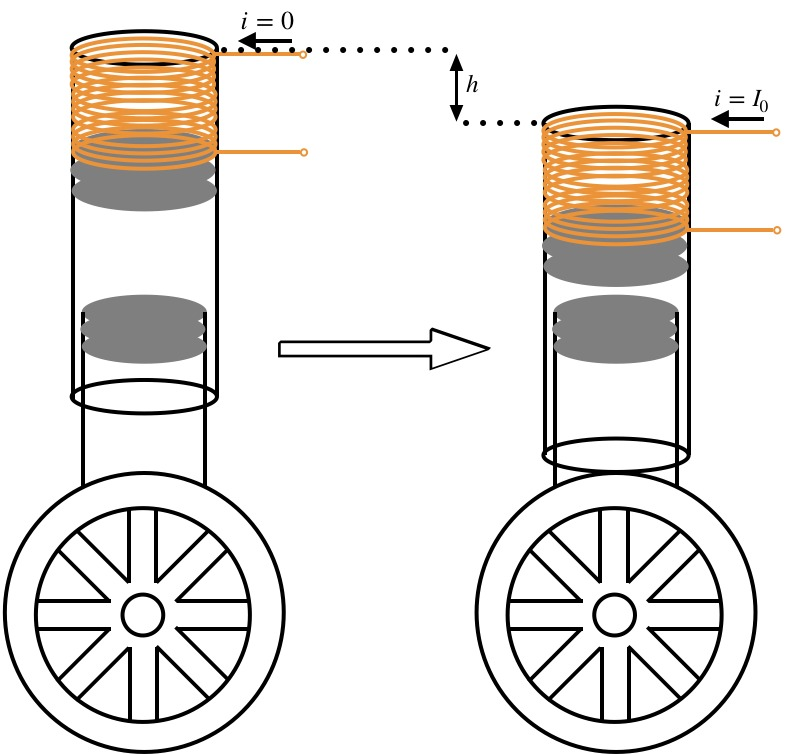
\includegraphics[width=0.48\textwidth]{suspension.jpeg}
    \caption{Designed Suspension System}\label{fig:suspension}
\end{figure}

\section{PROJECT DESCRIPTION}
Electromagnetic car suspension system with repulsive magnets as damping element, along with default height adjustment.    

\section{WORK PLAN}
Prior to finalizing the project proposal, a small experiment has been conducted in order to observe the applicability aspect. By passing current through a coil, wounded around a screw, we observed the effects of electromagnetism, which gave us a superficial intuition about the project. After being convinced that we can manage to achieve the proposed task, we finalized our proposal and outlined the work plan as follows.

\begin{enumerate}
    \item Theoretically calculate the magnetic field that we can obtain by passing current through a solenoid, and the resulting attractive/repulsive forces when we put this solenoid in an external magnetic field generated by permanent magnets.
    \item Build a test car that can demonstrate the passive suspension effect with the repulsive magnets as damping elements. 
    \item With additional coils wound to each suspension unit, acquire adjustable default height for the car (see Fig.~\ref{fig:suspension}).
    \item Add a controller to individually control each suspension unit.
\end{enumerate}
Since the following steps will not contribute to the electromagnetics part of the project, they are kept as optional steps for better demonstration. Additional implementation steps:
\begin{enumerate}
    \setcounter{enumi}{4}
    \item Control suspension height via bluetooth module (OPTIONAL).
    \item Add bluetooth control to the test car (OPTIONAL).
\end{enumerate}

\section{LIST OF EQUIPMENT}
\begin{itemize}
    \item Neodymium Magnets
    \item Syringes (as suspension pipe)
    \item Handmade Solenoids (0.5mm Copper Wire)
    \item Motor Driver with H-Bridge (LN298N)
    \item Power Source (Li-Po Battery or Power Supply)
    \item Microcontroller (Arduino)
    \item Bluetooth Module (HC-05)
    \item Toy Car Chassis and Wheels
\end{itemize}

% References
\printbibliography{}

\end{document}